\documentclass[12pt]{article}
\usepackage[scaled]{helvet}
\renewcommand\familydefault{\sfdefault} 
\usepackage[T1]{fontenc}

\usepackage[english]{babel}
\usepackage[utf8]{inputenc}
\usepackage{amsmath}
\usepackage{bm}
\usepackage{parskip}
\usepackage{hyperref}
\usepackage{graphicx}
\usepackage{listings}
\usepackage{xcolor}

\definecolor{Brown}{cmyk}{0,0.81,1,0.60}
\definecolor{OliveGreen}{cmyk}{0.64,0,0.95,0.40}
\definecolor{CadetBlue}{cmyk}{0.62,0.57,0.23,0}
\definecolor{lightlightgray}{gray}{0.9}

\lstset { %
    language=C++,
    %backgroundcolor=\color{black!5}, % set backgroundcolor
    %basicstyle=\footnotesize,% basic font setting
	basicstyle=\ttfamily,                   % Code font, Examples: \footnotesize, \ttfamily
	keywordstyle=\color{OliveGreen},        % Keywords font ('*' = uppercase)
	commentstyle=\color{gray},              % Comments font
	backgroundcolor=\color{lightlightgray},
	tabsize=4,
	frame=single,
}

\title{\textbf{Practical 6: Rigid Bodies, part 1 }}
\author{Babis Koniaris}
\date{}

\begin{document}
\maketitle

\begin{center}
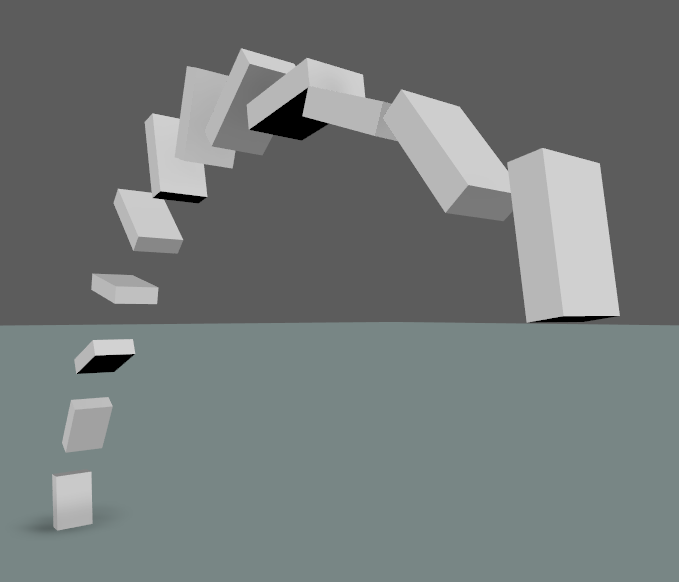
\includegraphics[width=\textwidth]{p6-teaser.png}
\end{center}
\pagebreak

\section*{Introduction}

The goals of this practical are to:

\begin{itemize}
\item Revise our architecture to support the addition of rigid bodies
\item Simulate rigid body rotations
\item Carry out simple collision detection between a rigid body (cuboid) and a plane
\end{itemize}

\section*{Architecture changes}

To assist with the requirements of rigid bodies, a slightly modified project is provided for you: ``04\_rigid\_body\_framework''. There are only a few key differences compared to the previous framework:

\begin{itemize}
\item The RigidBody class (declared in PhysicsObject.h) is derived from the Particle class \footnote{In production code we would not do this, as inheritance represents an ``is-a'' relationship, but the rigid body is not a particle. It is implemented here like this for convenience and framework code brevity.} and adds further functionality (such angular velocity and inverse inertia) to be used for rigid body simulation. 
\end{itemize}

You can copy over relevant code from your previous projects, so that your timestep and integration functionality is already implemented, although we won't be using Hooke forces anymore. In these practicals we will be revisiting collision detection, response and integration, to suit the nature of rigid bodies.

\section*{Tasks}

\subsection*{Task 1: Port integration and timestep to new project}

Before you start working on rigid bodies, make sure that this new project again includes integration and timestep code. As a first step, you should replace the single bouncing particle with a RigidBody. Because a RigidBody is derived from Particle, there should be no issue with the code and no different behaviour: every function that takes ``Particle\&'' as an argument will still work, as a RigidBody can be safely cast to its parent class: Particle. Set the rigid body to use the "box" mesh, and apply a scale and position of your choosing, e.g. $(1,2,1)$ and $(0,5,0)$ respectively. 

\textbf{Task 1: Port previous code so that you have a RigidBody object falling from gravity, using previous integration and timestep code.}

\subsection*{Task 2: Simulate the rotation of the rigid body}

Now it's time to add some rotation, with angular velocity. You should have 2 different scenarios:

\begin{itemize}
\item A rigid body with an initial angular velocity with non-zero magnitude.
\item A rigid body with zero angular velocity but some angular acceleration, that can be toggled on and off using a key. For example, by pressing K you enable the acceleration, and used at every simulation step to calculate the new velocity, but when you press K again the acceleration becomes zero, but the velocity remains as-is.
\end{itemize}

To avoid distractions, do \emph{not} apply gravity for this task. To utilise the angular values, we need to update the integration code. But what will the effect be? Just as we called "particle.SetPosition(position)" in our integration code, for the angular values we need to update the \emph{orientation} of the object. We can do that using the function "PhysicsBody::SetOrientation(mat4 orientation)" which we can call because the RigidBody is derived from the PhysicsBody. So, how do we obtain the orientation matrix from the angular quantities? With a combination of integration code and glm helper functions:

\begin{minipage}{\linewidth}\begin{lstlisting}
// dt: deltaTime, angAcc: angular acceleration
// integration (rotation)
auto newAngVel = rb.AngularVelocity() + dt * angAcc;
rb.SetAngularVelocity(newAngVel);
// create skew symmetric matrix for w
glm::mat3 angVelSkew = glm::matrixCross3(newAngVel);
// create 3x3 rotation matrix from rigidBody matrix
glm::mat3 R = glm::mat3(rb.Orientation());
// update rotation matrix
R += dt*angVelSkew*R;
R = glm::orthonormalize(R);
rb.SetOrientation(glm::mat4(R));
\end{lstlisting}\end{minipage}

\textbf{Task 2: Show two floating rigid bodies spinning side by side: one using a constant angular velocity while the other using angular acceleration that can be turned on and off by a key.}

\subsection*{Task 3: Collision detection}

Rotating a solid body was easy. What is not so easy is to compute by how much it should rotate and translate depending on the forces, torques and impulses applied to the body, and on what part of the body they are applied to. This is crucial to the implementation of convincing collisions but it is not on today's session. We will take care of this in the next couple of weeks. This week, let's address the first part of the collision problem: collision \emph{detection}, and more specifically of collisions between a solid body and a horizontal plane. 

\textbf{Task 3: Detect when the mesh of a rigid body object collides with the ground plane.}

Important information:

\begin{itemize}
\item You have access to the list of mesh vertex positions, stored in the MeshData structure, by accessing: rigidBody.GetMesh()->Data().positions.data
\item The mesh vertex positions are stored in local space. For your simulation, you need the coordinates in world space, so you have to multiply those vertices by the model matrix of the PhysicsObject: rigidBody.ModelMatrix(). Be aware of the occasional conversion to and from homogeneous coordinates.
\item Store the points of contact, as they can be more than one. An object can land on its tip, on an edge or on a face, each of which result in different numbers of contact points.
\item Consider adding a pause/resume button for your simulation, to observe what is going on
\end{itemize}

\subsection*{Further tasks}

If you can successfully detect collisions, you must be desperate to resolve the collision i.e., make the solid bounce in a realistic way. Try to implement a bouncing behaviour that seems reasonable to you. Start by making it bounce as it would if it were a particle and then consider how the angular velocity should be affected by collisions. Should it be reversed? Does it depend? What does it depend on? Reflecting on this problem will help you understand the solution when it is presented to you ...

\section*{Deliverables}

Nothing is assessed this week, but part of the work  (task 3) will be part of the assessed deliverables of a future practical.

\end{document}